\section{Theoretical insights}

\subsection{Covariate shift}
\begin{example} %[Covariate shift]
\label{ex_covshift}
%So far we have considered the isotropic model where $\Sigma_1 = \Sigma_2$.
%This setting is relevant for settings where different tasks share the same input features such as multi-class image classification.
%In general, the covariance matrices of the two tasks may be different such as in text classification.
To illustrate the effect of covariate shift, we consider a similar setting as in Example \ref{ex_sample_ratio}, such that \eqref{para_rel} holds. In Proposition \ref{lem_hat_v}, we have seen that the global minimizer $\hat a$ is close to 1 up to a small error. Hence we take $a=1$ in \eqref{lem_cov_shift_eq}, and study the asymptotic limit
$$\ell_{\var}(M):= \frac{\sigma^2}{n_1+n_2}\bigtr{  \frac{1}{a_1(M) \cdot M^\top M + a_2(M)  }  }, $$
where $ M=(\Sigma^{(1)})^{1/2}(\Sigma^{(2)})^{-1/2}$, and $a_1(M)$ and $a_2(M)$ are defined through \eqref{eq_a12extra}.
We compare different choices of $M$ that are scaled to have the same determinant. More precisely, for a fixed $\mu>0$ we define
\begin{align*}
		\cS_{\mu}\define\bigset{M \left| \prod_{i=1}^p \lambda_i = \mu^p, \tau \le \lambda_p \le \lambda_1 \le \tau^{-1}\right.}.
\end{align*}
%belong to the following bounded set.
%Let $\lambda_i$ be the $i$-th singular value of $M$.
%let $\mu_{\min} < \mu < \mu_{\max}$ be fixed values that do not grow with $p$.
%\vspace{-0.025in}
%{\small}
%	We assume that $\beta_1$ and $\beta_2$ are generated following the isotropic model with $d = 0$.
%\begin{proposition}[Covariate shift]\label{prop_covariate}
%	Assume that $\Psi(\beta_1, \beta_2) = 0$ and $\rho_1, \rho_2>1$.
%	Let $g(M)$ denote the prediction loss of $\hat{\beta}_t^{\MTL}$ when $M = \Sigma_1^{1/2}\Sigma_2^{-1/2} \in\cS_{\mu}$.
%	We have that
%	{\small\[ g(\mu\id) \le \bigbrace{1+ \bigo{{\rho_2}/{\rho_1}  }} \min_{M\in\cS_{\mu}} g(M). \]}
%\end{proposition}
%This proposition shows that when source/target sample ratio is large, then having no covariate shift is optimal.
%The proof of Proposition \ref{prop_covariate} is left to Appendix \ref{app_proof_33}.
%We now prove Proposition \ref{prop_covariate}, which shows that $\te(\hat{\beta}^{\MTL})$ is minimized approximately when $M$ is a scalar matrix where there is enough source data.
Our first observation is that if $n_1 \gg n_2$, i.e. there is enough source data compared to the target data, then $\ell_{\var}(M)$ is minimized approximately when $M$ is a scalar matrix.
%\begin{proof}[Proof of Proposition \ref{prop_covariate}]
%Let
%$$M_0:=\argmin_{M\in \cal S_{\mu}}g(M).$$
%We now calculate $g(M_0)$. With the same arguments as in Lemma \ref{lem_hat_v}, we can show that \eqref{hatv_add1} holds. Moreover, if the parameters are chosen such that $p^{-1+c_0} \sigma^2 \le \kappa^2  \le p^{-\e_0-c_0}\sigma^2$ as in \eqref{choiceofpara}, we can simplify
%\be \nonumber
%\begin{split}
%g(M_0)&=(1+\OO(p^{-\e}))\cdot \sigma^2  \bigtr{\Sigma_2(X_1^{\top}X_1  + X_2^{\top}X_2)^{-1} }  ,
%\end{split}
%\ee
%with high probability for some constant $\e>0$. In fact, Lemma \ref{lem_hat_v} was proved assuming that $M=\id$, but its proof can be easily extended to the case with general $M\in \cal S_{\mu}$ by using that $ \mu_{\min}\le \lambda_p(M)\le \lambda_1(M)\le \mu_{\max}$. We omit the details here.
%
%Now using Lemma \ref{lem_cov_shift}, we obtain that with high probability,
%\begin{align}\label{gvar_extra}
%g(M_0)= \frac{\sigma^2}{\rho_1+\rho_2}\cdot \frac1p\tr\left( \frac{1}{a_1(M_0)\cdot M_0^\top M_0 + a_2(M_0)}\right) \cdot \left(1 +\OO(p^{-\e})\right).
%\end{align}
In fact, from equation \eqref{eq_a12extra}, we obtain the following estimates on $ a_1(M)$ and $a_2(M)$ for any $M\in \cal S_\mu$:
\be\label{est_a12extra}
 a_1(M) = \frac{n_1+\OO(p)}{n_1+n_2},\quad a_2(M) =\frac{n_2+\OO(p)}{n_1+n_2}.
\ee
Inserting \eqref{est_a12extra} into $\ell_{\var}(M)$, we obtain that
%and using $ M_0^\top M_0\succeq \mu_{\min}^2$, we obtain that with high probability,
%\begin{align}\label{approximateteM}
%\left(1+\frac{\rho_2}{(\rho_1-1)\mu_{\min}^2}\right)^{-1}h(M_0) \cdot \left(1 - \OO(p^{-\e})\right) \le g(M_0) \le h(M_0) \cdot \left(1 +\OO(p^{-\e})\right),
%\end{align}
%where
$$\ell_{\var}(M)= \left[ 1+\OO\left(\frac{n_2}{n_1}\right)\right] \cdot \frac{\sigma^2}{n_1} \tr\left( \frac{1}{M^\top M}\right) .$$
%With these two bounds, we can easily conclude \eqref{approxteM}.
%
%We have that the test error satisfies
%\be\label{approxteM}  te(M)\left(1 -  \frac{n_2}{n_1-p} \frac{1}{\lambda_p^2 + \frac{n_2}{n_1-p}}\right)  \le  \frac{\sigma^2}{n_1+n_2}\tr\left( \frac{1}{a_1M^\top M + a_2}\right) \le te(M),\ee
%where $\lambda_p$ is the smallest singular value of $p$ and
%$$te(M):= \frac{\sigma^2}{a_1(n_1+n_2)}\tr\left( \frac{1}{M^\top M}\right) .$$
%Moreover, for all $M$ satisfying \eqref{GMcons}, the minimum of $te(M)$ is attained when $M= a\id$.
By AM-GM inequality, we observe that
$$\tr\left( \frac{1}{M^\top M}\right) = \sum_{i=1}^p\frac{1}{\lambda_i^2}$$
is minimized when $\lambda_1 = \cdots\lambda_p=\mu$ under the restriction $\prod_{i=1}^p\lambda_i =\mu^p$. Hence in this case, $M=\mu \id_{p\times p}$ is approximately the optimal choice.

%Hence we get that
%\be\label{AMGM} h(M_0) \le \frac{\sigma^2}{\mu^2 (\rho_1+\rho_2)a_1(M_0)}.\ee
%
%On the other hand, when $M=\mu \id$, applying Lemma \ref{lem_cov_shift} we obtain that with high probability,
%\begin{align}\label{gvar_extra2}
%\begin{split}
%g(\mu \id)&= \frac{\sigma^2}{\rho_1+\rho_2}\cdot \frac1p\tr\left( \frac{1}{\mu^2 a_1 (\mu\id) + a_2(\mu\id)}\right) \cdot \left(1 +\OO(p^{-\e})\right)\\
%&\le \frac{\sigma^2}{\mu^2(\rho_1+\rho_2)a_1 (\mu\id)}.
%\end{split}
%\end{align}
%Combining \eqref{est_a12extra}, \eqref{approximateteM}, \eqref{AMGM} and \eqref{gvar_extra2}, we conclude the proof.
%, we conclude that the sum $\sum_{i=1}^p\lambda_i^{-1}$ is smallest when $\lambda_1=\cdots=\lambda_p = a$.
%\end{proof}


\iffalse
For large enough $p$,
%in the left hand side of equation \eqref{lem_cov_shift_eq}:
\begin{align*}
	\bigtr{\Sigma^{(2)} \hat{\Sigma}^{-1}} &\rightarrow \frac{1}{n_1 + n_2} \bigtr{\Sigma^{(2)} (a_1 \Sigma^{(1)} + a_2 \Sigma^{(2)})^{-1}}
	= \frac{1}{n_1 + n_2} \bigtr{(a_1 M^{\top} M + a_2 \id)^{-1}}.
\end{align*}
%As we are going to show later, covariate shift is accurately captured by the spectrum of $\Sigma^{1/2}\Sigma^{-1/2}$.
Hence the variance limit depends on the spectrum of $M$. % To be clear, for this example we assume that the bias is $0$.
\fi

%Our second example focuses on how varying covariate shifts impacts the \textit{variance} limit in equation \eqref{lem_cov_shift_eq}.
%Our first observation is that:
However, we now use an example to show that the above observation fails when $n_1$ is comparable to $n_2$. We take $\mu =1$, and consider the subset of covariate shift matrices satisfying $M=M^{-1}$. In other words, half of the singular values of $M$ satisfy that $\lambda_1 \ge \lambda_2\ge \cdots \ge \lambda_{p/2} \ge 1$, while the other half eigenvalues are $\lambda_{p/2}^{-1}\ge \cdots \ge \lambda_2^{-1} \ge \lambda_1^{-1}$. When $\lambda_1/\lambda_{p/2} = 1$, we have $M=\id_{p\times p}$ and there is no covariate shift.
%while as As $\lambda$ increases, the severity of covariate shift increases.
We claim the following dichotomy.
\begin{enumerate}
	\item If $n_1 \ge n_2$, then the variance limit is smallest when there is no covariate shift.
	\item If $n_1 < n_2$, then the variance limit is largest when there is no covariate shift.
\end{enumerate}
We explain why the above dichotomy happens. We can write the variance limit as
$$\ell_{\var}(M)=\frac{\sigma^2}{ n_1+n_2 }\sum_{i=1}^{p/2}\left( \frac{1}{\lambda_i^{2} a_1 + a_2} + \frac1{\lambda_i^{-2} a_1 + a_2} \right) .$$
When $M=\id_{p\times p}$, by the first equation of \eqref{eq_a12extra}, we have
$$\ell_{\var}(\id_{p\times p})=\frac{\sigma^2}{ n_1+n_2 }\sum_{i=1}^{p/2} \frac{2}{1-\gamma} , $$
where we abbreviate $\gamma:=p/(n_1+n_2)$. Then using $a_1+a_2=1-\gamma$, through a direct calculation we find that %we can calculate that
\begin{align*}
\ell_{\var}(M) - \ell_{\var}(\id_{p\times p})%&= \frac{\sigma^2 \gamma}{2(1-\gamma)} (\lambda^2-1)a_1\cdot \bigbrace{  \frac{1}{ -a_1(\lambda^2-1)+(1-\gamma)\lambda^2 } - \frac{1}{a_1(\lambda^2-1) + (1-\gamma)}} \\
&= \frac{\sigma^2 }{ n_1+n_2-p} \sum_{i=1}^{p/2} \frac{(\lambda_i^2-1)^2 a_1(M) \left[ a_1(M) - a_2(M)\right] }{[a_1(M)+\lambda_i^2 a_2(M)][\lambda_i^2 a_1(M)+a_2(M)]} .
\end{align*}
%in this example is equal to
%$\frac{p}{2(n_1 + n_2)} f(\lambda)$, where
%\[ f(\lambda) = {(\lambda^{-2} a_1 + a_2)^{-1} + (\lambda^2 a_1 + a_2)^{-1}}. \]
%Using the fact that $a_1 + a_2 = 1 - \frac{p}{n_1 + n_2}$, we can verify
%\begin{align*}
%	f(\lambda) - f(1) &= \left(\lambda^2 a_1 + \frac{n_1 + n_2 - p}{n_1 + n_2} - a_1\right)^{-1} \\
%	&+ \left(\lambda^{-2} a_1 + \frac{n_1 + n_2 - p}{n_1 + n_2} - a_1\right)^{-1} \\
%	&- \frac{2(n_1 + n_2)}{n_1 + n_2 - p} \\
%	&= \left(2a_1 - \frac{n_1 + n_2-p} {n_1 + n_2 }\right)  g(\lambda, a_1), %\cdot (\lambda^2-1)^2
%\end{align*}
%\begin{align*}
%	f(\lambda) - f(1) &= \left(2a_1 - \frac{n_1 + n_2-p} {n_1 + n_2 }\right)  g(\lambda, a_1), %\cdot (\lambda^2-1)^2
%\end{align*}
%where $g(\lambda, a_1) \ge 0$.
%and can be derived from algebraic calculations (details omitted).
We claim that $a_1(M) > a_2 (M)$ if and only if $n_1 > n_2$, which then explains the dichonomy. In fact, if $a_1>a_2$, then the first equation in \eqref{eq_a12extra} gives that $a_1> (1-\gamma)/2$, and the second equation in  \eqref{eq_a12extra} gives that
\begin{align*}
 \frac{n_1}{n_1 + n_2} &> a_1 + \frac{1}{n_1+n_2} \sum_{i=1}^{p/2}\left(\frac{\lambda_i^2}{\lambda_i^2+1}+\frac{\lambda_i^{-2}}{\lambda_i^{-2}+1}\right) = \frac{1-\gamma}{2}+\frac{\gamma}{2}=\frac{1}{2}.
\end{align*}
%\begin{align*}
% \frac{n_1}{n_1 + n_2} &=a_1 + \frac1{n_1 + n_2}\cdot \bigbrace{\sum_{i=1}^p \frac{\lambda_i^2 a_1}{\lambda_i^2 a_1 + a_2}} \\
%	&> a_1 + \frac{p}{2(n_1+n_2)} \left(\frac{\lambda^2}{\lambda^2+1}+\frac{\lambda^{-2}}{\lambda^{-2}+1}\right) =\frac{1}{2}.
%\end{align*}
This implies $n_1>n_2$. The other direction follows from a similar argument. % Similarly, if $a_1<a_2$, equations  \eqref{eq_a12extra000} and  \eqref{eq_a12extra} give that $a_1 < \frac{n_1 + n_2-p}{2 (n_1 + n_2)}$ and $n_1<n_2$. Thus, we conclude that $f(\lambda) \ge f(1)$ if and only if $n_1 \ge n_2$.
\end{example}

\iffalse
%FY: Below was the word explanation. I still think the above simple proof is clearer.
In fact, due to the fact that $M=M^{-1}$, $a_1$ and $a_2$ play symmetric roles in equations \eqref{eq_a12extra000} and \eqref{eq_a12extra}.
Hence, when $n_1 \ge n_2$, we have that $a_1 \ge a_2$, hence $a_1 \ge \frac{1}{2}(1 - \frac{p}{n_1 + n_2 - p}) = \frac{n_1 + n_2}{2 (n_1 + n_2 - p)}$.
The other case when $n_1 < n_2$ is similar.
A formal proof follows easily from the self-consistent equations \eqref{lem_cov_shift_eq} and we omit the details.
Thus, we conclude that if $n_1 \ge n_2$, then $f(\lambda) > f(1)$.
If $n_1< n_2$, then $f(\lambda)< f(1)$.
\fi



For the bias limit, we have the following proposition.

\begin{proposition}\label{prop_main_RMT}
%The bias equation \eqref{Lbias} satisfies the following limit with high probability: Let $S$ be an arbitrary subset of the unit sphere in dimension $p$ whose size is polynomial in $p$, for any unit vector $w\in S$,
Under Assumption \ref{assm_big1}, for any small constant $c>0$ and large constant $C>0$, there exists a high probability event $\Xi$, on which the following estimate  holds for $L_{\bias}(a)$ in \eqref{Lbias}:
			\begin{align}
				& \bigabs{ L_{\bias}(a) -   (\beta^{(1)}- a\beta^{(2)} )^\top (\Sigma^{(1)})^{1/2} \Pi(a)(\Sigma^{(1)})^{1/2} (\beta^{(1)}- a\beta^{(2)})   }  \nonumber\\
				& \le \left[\left( 1+\sqrt{\frac{p}{n_1}}\right)^4 - 1 +\OO\left( n_1^{-1/2+2/\varphi + c}\right)\right] \frac{n_1^2 \lambda_1^2 \left\|(\Sigma^{(1)})^{1/2} \left(\beta^{(1)}- a\beta^{(2)}\right) \right\|^2}{  [(\sqrt{n_1}-\sqrt{p})^2 \lambda_p^2+ (\sqrt{n_2}-\sqrt{p})^2]^2}  \nonumber\\
				& + p^{-C} \left[\| \beta^{(1)}\|^2 + \| \beta^{(2)}\|^2 \right], \label{lem_cov_derv_eq}
			\end{align}
%			\begin{align}\label{lem_cov_derv_eq}
%				\bigabs{ L_{\bias}(a) - \left\|\frac{n_1}{n_1+n_2}  \frac{\left[a_3 M(a)^\top M(a) + (a_4 + 1) \right]^{1/2}}{ a_1 M(a)^\top M(a) + a_2 } M(a)^\top (\Sigma^{(1)})^{1/2} \left(\beta^{(1)}- a\beta^{(2)}\right)\right\|^2   } \le  \frac{p^{-c_{\varphi}}}{(n_1+n_2)^2},
%			\end{align}
				uniformly in all $a\in \R$. Here $\lambda_1$ and $\lambda_p$ are respectively the largest and smallest singular values of $M(a)$, $\Pi(a)$ is a $p\times p$ matrix defined as
				$$\Pi(a):=\frac{n_1^2}{(n_1+n_2)^2}  M(a)  \frac{a_3 M(a)^\top M(a) + (a_4 + 1) }{[a_1 M(a)^\top M(a) + a_2 ]^2} M(a)^\top  ,$$
				 and $(a_{3},a_4)$ is the solution of the following system of equations % with $b_k = \frac1{p}\sum_{i=1}^p \frac{\lambda_i^{2k}} {(\lambda_i^2 a_1 + a_2)^2}$, for $k = 0, 1, 2$:
		\be  \label{eq_a34extra}
		\begin{split}
				& a_3 + a_4 = \frac{1}{n_1 + n_2}\sum_{i=1}^p \frac{1}{\lambda_i^2 a_1 + a_2}, \\
				& a_3 + \frac{1}{n_1 + n_2} \sum_{i=1}^p \frac{\lambda_i^2 (a_2 a_3-a_1 a_4 )}{(\lambda_i^2 a_1 + a_2)^2} = \frac{1}{n_1 + n_2} \sum_{i=1}^p \frac{\lambda_i^2 a_1}{(\lambda_i^2 a_1 + a_2)^{2}},
%				\left(\frac{\rho_1}{a_1^{2}} -  b_2  \right)\cdot  a_3 -  b_1 \cdot  a_4 = b_1,\quad \left(\frac{\rho_2}{a_2^{2}}-  b_0\right)\cdot  a_4 - b_1 \cdot  a_3
%				= b_0.
			\end{split}
			\ee
			where we recall that $(a_1,a_2)$ is the solution of \eqref{eq_a12extra}.
\end{proposition}

Note that the first error term on the right-hand side of \eqref{lem_cov_derv_eq} is typically smaller than the main term $ (\beta^{(1)}- a\beta^{(2)} )^\top (\Sigma^{(1)})^{1/2} \Pi(a)(\Sigma^{(1)})^{1/2} (\beta^{(1)}- a\beta^{(2)})  $ by a factor of $\OO(\sqrt{p/n_1} + n_1^{-1/2+2/\varphi + c})$. Hence \eqref{lem_cov_derv_eq} only gives an exact asymptotic limit in the regime $n_1\gg p$. Moreover, by equations \eqref{eq_a12extra} and \eqref{eq_a34extra} we have
$$a_1 =\frac{n_1}{n_1+n_2} + \OO\left( \frac{p}{n_1+n_2}\right), \quad a_3 =\frac{n_3}{n_1+n_2} + \OO\left( \frac{p}{n_1+n_2}\right),$$
and
$$a_3 =\OO\left( \frac{p}{n_1+n_2}\right),\quad a_4 =\OO\left( \frac{p}{n_1+n_2}\right).$$
Using these estimates, it is easy to check that
\begin{align}
& (\beta^{(1)}- a\beta^{(2)} )^\top (\Sigma^{(1)})^{1/2} \Pi(a)(\Sigma^{(1)})^{1/2} (\beta^{(1)}- a\beta^{(2)})   \nonumber \\
&=\left\| (\Sigma^{(2)})^{1/2}\frac{1}{a^2\Sigma^{(1)}+\Sigma^{(2)}} a \Sigma^{(1)} \left(\beta^{(1)}- a\beta^{(2)}\right) \right\|^2 + \OO\left( \frac{p\left\|\beta^{(1)}- a\beta^{(2)}\right\|^2}{n_1+n_2}  \right)  . \label{bias_LLN}
\end{align}
Hence \eqref{lem_cov_derv_eq} is consistent with the result obtained by replacing $ (X^{(1)})^\top X^{(1)}$ and $ (X^{(2)})^\top X^{(2)}$ with $n_1\Sigma^{(1)}$ and $n_2\Sigma^{(2)}$, respectively, in $L_{\bias} (a) $ using the law of large numbers in the regime $n_1\gg p$. However, simulations show that our estimate \eqref{lem_cov_derv_eq} is more precise than the first term on the right-hand side of \eqref{bias_LLN}.

\begin{remark}
%First, our result in Corollary \ref{cor_MTL_loss} involves an error term that scales down with $n_1$.
%Tightening this error bound requires showing the limit of $\normFro{({Z^{(1)}}^{\top} Z^{(1)} + {Z^{(2)}}^{\top} Z^{(2)})^{-1} {Z^{(1)}}^{\top} Z^{(1)}}^2$ for two isotropic sample covariance matrices.
%This requires studying the asymptotic singular values distribution of the non-symmetric matrix $({Z^{(1)}}^{\top} Z^{(1)})^{-1}{Z^{(2)}}^{\top} Z^{(2)}+\id$, which is still an open problem in random matrix theory.
%\begin{remark}
The main error in Proposition \ref{prop_main_RMT} comes from approximating $(Z^{(1)})^\top Z^{(1)}$ by $n_1\id_{n_1\times n_2}$ using Corollary \ref{fact_minv} in the supplement \cite{MTL_suppl}. In order to improve this estimate and obtain an exact asymptotic result, one needs to study the singular value distribution of the  random matrix $\cal X + a^2$ for any fixed $a\in \R$, where $\cal X:=[(X^{(1)})^{\top}X^{(1)}]^{-1}(X^{(2)})^{\top}X^{(2)}$. We remark that the eigenvalues of $\cal X$ have been studied in the name of Fisher matrices \cite{Fmatrix}. However, since $\cal X$ is not symmetric, its singular values are different from its eigenvalues. To the best of our knowledge, the asymptotic singular value behavior of $\cal X$ is still an open problem in random matrix theory, and the study of the singular values of $\cal X + a^2$ will be even harder. We leave this problem to future study.

We also remark for the general case with covariate shift, the method in Section \ref{sec_sizeratio} for the bias term also fails, because we cannot reduce the problem into the free addition of two random matrices that are asymptotically freely independent.
%\end{remark}
\end{remark}





%{\cob The idea of proof: proved using free probability; can also use polynomials of random matrices.}

%Now we use the following example to illustrate the effect of varying sample sizes on the predication loss of the HPS estimator.



To describe quantitively the bias-variance tradeoff phenomenon and the effect of varying sample sizes on the predication loss, we consider a \emph{random-effect model}, which has been studied for  single-task linear regression and ridge regression (see e.g. \cite{dobriban2020wonder,dobriban2018high}).




 %{How does hard parameter sharing scale with sample sizes and covariate shift $M$?} One can see that the variance limit depends intricately on both tasks' samples sizes and covariate shift. Next, we illustrate how varying them impact the prediction loss.
\begin{example}%[Sample sizes]
\label{ex_sample_ratio}
	%We first consider the impact of varying sample sizes.
	%Consider the random-effect model from Section \ref{sec_same}, with both tasks having an isotropic population covariance matrix.
	%We again consider the random effect model in Example \ref{ex_same_cov} with $t=2$.
	Suppose each $\beta^{(i)}$ consists of two random components, one that is shared among the two tasks and one that is task-specific. More precisely, we let
$$\beta^{(i)}=\beta_0 +\wt \beta^{(i)},\quad i=1,2, $$
where $\beta_0$ denotes the shared component, %whose entries are i.i.d. Gaussian random variables of mean zero and variance $p^{-1}\kappa^2$,
and $\wt \beta^{(i)}$ denotes the $i$-th
%Let $\beta^{(i)}$ be equal to $\beta_0$ plus a
task-specific component whose entries are i.i.d. Gaussian random variables of mean zero and variance $p^{-1} d^2$. First, we show that if $\|\beta_0\|^2 \gg d^2$, then the global minimizer $\hat a$ of the function $g(a)$ in \eqref{eq_mtl_A12} is close to $1$.
	The proof of Proposition \ref{lem_hat_v} will be given in Appendix \ref{app_iso_cov_prop}.

	\begin{proposition}\label{lem_hat_v}
%Suppose the assumptions of Lemma \ref{prop_model_shift_tight} hold. Assume that $ \kappa^2 \sim pd^2 \sim \sigma^2$ are of the same order.
Suppose Assumption \ref{assm_big1} and the above setting of random effect model hold. %in Example \ref{ex_same_cov} hold.
Suppose that for a constant $c_0>0$,
	\be\label{para_rel}
	 \|\beta_0\|^2 \ge p^{c_0}d^2 +p^{-1/2+c_0}\sigma^2.
	\ee
 Then we have that for any small constant $c>0$ and large constant $ C>0$,
	%Let $c$ be a sufficiently small fixed constant.
	%In the setting of Corollary \ref{cor_MTL_loss},
%There exists a constant $C>0$ such that
	\be\label{hatw_add1}
	 \hat a =1+ \OO\left(\frac{d^2}{\|\beta_0\|^2} + p^{-1/4+c} \frac{d+\sigma}{\|\beta_0\|} + p^{-C}\right) \quad \text{w.h.p.}
	\ee
\end{proposition}
%Suppose every $\beta^{(i)}$ consists of two random components, one that is shared among all tasks and one that is task-specific.
%%Thus, each task contributes a certain amount to the shared component and injects a task-specific bias.
%More precisely, %we have
%$$\beta^{(i)}=\beta_0 +\wt \beta^{(i)},\quad i=1,2,\cdots, t,$$
%where $\beta_0$ denotes the shared component, %whose entries are i.i.d. Gaussian random variables of mean zero and variance $p^{-1}\kappa^2$,
%and $\wt \beta^{(i)}$ denotes the $i$-th
%%Let $\beta^{(i)}$ be equal to $\beta_0$ plus a
%task-specific component whose entries are i.i.d. Gaussian random variables of mean zero and variance $p^{-1} d^2$.

We emphasize that unlike Theorem \ref{cor_MTL_loss}, for Proposition \ref{lem_hat_v} we do not assume $\Sigma^{(1)}=\Sigma^{(2)}$ and the Gaussian distributions of the entries of $Z^{(1)}$ and $Z^{(2)}$. Combining Lemma \ref{lem_HPS_loss}, Theorem \ref{cor_MTL_loss} and Proposition \ref{lem_hat_v}, and using  that $\|\beta^{(1)}-\beta^{(2)}\|^2 = (2+\oo(1))d^2$ with high probability, the predication loss $L(\hat{\beta}_2^{\MTL}(\hat a)) $ is approximately equal to
$$\ell(n_1,n_2)= \sigma^2 \cal L_1(1) +   2d^2 \cal L_2(1)= \frac{p\sigma^2}{n_1+n_2-p} +  2d^2  \frac{n_1^2 (n_1+n_2-p)+p n_1n_2}{(n_1+n_2)^2(n_1+n_2-p)}, $$
with high probability, where in the second step we obtain $\cal L_1(1)$ and $\cal L_2(1)$ through direct calculations.
Now we compare $\ell(n_1,n_2)$ with \eqref{L_STL_simple01}. First, we notice that the variance term $\sigma^2 \cal L_1(1)$ is smaller than $L(\hat{\beta}_2^{\STL} )$, while the bias term always increases (because the bias in single-task linear regression is zero). This gives a \emph{bias-variance tradeoff} for the predication loss of the HPS estimator. Second, calculating the derivative with respect to $n_1$, it is not hard to see that the variance term always decreases as $n_1$ increases, while the bias term always increases with $n_1$. Hence how the performance of the HPS estimator changes with respect to $n_1$ also depends on an intricate bias-variance tradeoff.

Now fix an $n_2$, we study the bias-variance tradeoff with respect to $n_1$ using the following function of $\rho:=\rho_1+\rho_2$, which is $L(\hat{\beta}_2^{\STL} )-\ell(n_1,n_2)$ divided by $2d^2$:
$$h(\rho):=\frac{p }{n_2-p}\cdot \frac{\sigma^2}{2d^2}- \frac{\ell(\rho_1p , \rho_2p)}{2d^2}  = \frac{\rho-\rho_2}{(\rho-1)(\rho_2-1)}\cdot \frac{\sigma^2}{2d^2}- \frac{(\rho-\rho_2)^2 (\rho-1)+(\rho-\rho_2)\rho_2}{\rho^2(\rho-1)}  .$$
This function characterizes $L(\hat{\beta}_2^{\STL} )-L(\hat{\beta}_2^{\MTL}(\hat a)) $, and hence gives the quantitive information transfer from the source task to the target task.
First, we have positive (resp. negative) transfer if and only if $h(\rho)>0$ (resp. $h(\rho)<0$). Moreover, the sign of $h(\rho)$ is determined by the sign of the second order polynomial %which is equivalent to the following inequality:
\be\label{poly1} \left( \frac{1}{\rho_2-1}\cdot \frac{\sigma^2}{2d^2}-1 \right)\rho^2 + ( \rho_2+1)\rho - 2\rho_2 .\ee
We observe the following dichotomy. %\FY{add several plots to illustrate this dichotomy}
\begin{enumerate}
\item If $\frac{1}{\rho_2-1}\cdot \frac{\sigma^2}{2d^2}-1 >0$, then the polynomial \eqref{poly1} is positive for all $\rho\in (\rho_2+1,\infty)$, so that the transfer is always positive.

\item If $\frac{1}{\rho_2-1}\cdot \frac{\sigma^2}{2d^2}-1 < 0$, then we have the following cases.

\begin{itemize}
\item If $(\rho_2+1)^2 < 8\rho_2 \left( 1- \frac{1}{\rho_2-1}\cdot \frac{\sigma^2}{2d^2}  \right)$, the polynomial \eqref{poly1} is negative for all $\rho$, so that the transfer is always negative.

\item If $(\rho_2+1)^2 > 8\rho_2 \left( 1- \frac{1}{\rho_2-1}\cdot \frac{\sigma^2}{2d^2}  \right)$, the polynomial \eqref{poly1} has two positive roots, where one of them is always smaller than $\rho_2+1$. Hence if the larger root, say $\rho_c$, is smaller than $\rho_2+1$, then the transfer is always negative for $\rho\in (\rho_2+1,\infty)$; otherwise, there is a transition from positive transfer to negative transfer as $\rho$ crosses $\rho_c$.
\end{itemize}
\end{enumerate}
Second, we calculate the derivative of $h(\rho)$, and find that its sign  is determined by the sign of the third order polynomial
\be\label{poly2}
 \frac{1}{\rho_2}\cdot \frac{\sigma^2}{2d^2} \rho^3 - 2(\rho-\rho_2)(\rho-1)(\rho-2)   - (\rho_2-1)\rho .\ee
Then we observe the following dichotomy. %\FY{add several plots to illustrate this dichotomy}
\begin{enumerate}
\item If $\frac{1}{\rho_2}\cdot \frac{\sigma^2}{2d^2} > 2$, the polynomial \eqref{poly2} is always positive for all $\rho\in (\rho_2+1,\infty)$, so that the information transfer always increases as $n_1$ increases.

\item If $\frac{1}{\rho_2}\cdot \frac{\sigma^2}{2d^2} < 2$, the polynomial \eqref{poly2} is positive initially around $\rho=\rho_2+1$, and then becomes negative when $\rho$ crosses its unique root, say $\rho_c$, in $(\rho_2+1,\infty)$. Hence the information transfer achieves the global maximum at $\rho=\rho_c$.
\end{enumerate}

%where $w_0:={\sigma^2}/{2d^2}$ is the ratio between the model bias and the noise variance.
%and $$ h_1(\rho_1,\rho_2):= \frac{\rho_1}{(\rho_1+\rho_2-1)(\rho_2-1)},\quad h_2(\rho_1,\rho_2):= \frac{\rho_1^2 (\rho_1+\rho_2-1)+\rho_1\rho_2}{(\rho_1+\rho_2)^2(\rho_1+\rho_2-1)}.$$
\iffalse
Then whether $L(\hat{\beta}_2^{\MTL}(\hat a)) $ is larger or smaller than

Applying Theorem \ref{thm_main_RMT} to the above setting, we get that
	\begin{align*}
		\frac{1}{n_1 + n_2} \tr[\Sigma^{(2)} (a_1\Sigma^{(1)} + a_2\Sigma^{(2)})^{-1}]
		= \frac{1}{n_1 + n_2} \bigtr{((a_1 + a_2)\id_p)^{-1}}
		= \frac{p}{n_1 + n_2 - p},
	\end{align*}
	because $a_1 + a_2 = 1 - \frac{p}{n_1 + n_2}$ by equation \eqref{eq_a12extra}.
	%Similarly, for the bias limit, we solve the self-consistent equations \eqref{eq_a34extra} to get $a_3$ and $a_4$ after we have obtained $a_1, a_2$.
	Similarly, we can calculate the bias limit.
	Combined together, we obtain the following corollary of Theorem \ref{thm_main_RMT}.

In the above inequality, the $d^2$ scaling term is the bias limit and the $\sigma^2$ scaling term is the variance limit.
This result allows for a more concrete interpretation since the dependence on datasets' properties is explicit.
The proof of Corollary \ref{cor_MTL_loss} can be found in Appendix \ref{app_iso_cov}.
As a remark, %in equation \eqref{cor_MTL_error}, the predication loss $L(\hat{\beta}_2^{\MTL}) $ was obtained using the global minimizer $(\hat A,\hat B)$. B
by combining the bias and variance limits, we can also obtain a bias-variance tradeoff for any local minimizer of $f(A, B)$.
The proof is similar to Corollary \ref{cor_MTL_loss}, so we omit the details.

{\cor
For the variance term, using equation \eqref{lem_cov_shift_eq}, we obtain that
\be\label{eq_var111}\tr[\hat\Sigma^{-1}] = \tr\left[ \left((X^{(1)})^\top X^{(1)}  + (X^{(2)})^\top X^{(2)}\right)^{-1}\right]=\bigtr{\frac{(a_1 +a_2)^{-1}\id_{p\times p}}{n_{1}+n_2} }+\OO(p^{-c_\varphi})\ee
with high probability. Solving equation \eqref{eq_a12extra} with $\lambda_i\equiv 1$, $1\le i\le p$, we get that
	\begin{align}
		 a_1 = \frac{n_1(n_1 + n_2 - p)}{(n_1 + n_2)^2} ,\quad
		& a_2 = \frac{n_2(n_1 + n_2 - p)}{(n_1 +n_2)^2} . \label{simplesovlea12}
			\end{align}
Applying the above to equation \eqref{eq_var111}, we obtain that with high probability
\be\label{eq_var112}\tr[\hat\Sigma^{-1}]  = \frac{p}{n_1+n_2} \cdot \frac{n_1+n_2}{n_1+n_2-p}+\OO(p^{-c_\varphi})=  \frac{p}{n_1+n_2-p}+\OO(p^{-c_\varphi}).\ee
For the bias term,
}


Next, we use the bias-variance limits to study how varying sample sizes impacts HPS.
For example, imagine if we want to decide whether to collect more of task one's data or not, how does increasing $n_1$ affect the prediction loss?
We assume that $n_2$ is fixed for simplicity.
%Now we illustrate an interesting phenomenon that adding task one's samples helps task two initially, but may hurt eventually.
The variance limit in equation \eqref{cor_MTL_error} obvious decreases with $n_1$.
It turns out that the bias term always increases with $n_1$, which can be verified by showing that the bias limit's derivative is always nonnegative.
%As a function of the sample ratio, the limiting estimate always decreases first from $\frac{\sigma^2 p}{n_2 - p}$ with $n_1$ being zero, and then increases to $d^2$ when $n_1$ goes to infinity.
%We describe a sketch of the proof.
By comparing the derivative of the bias and variance limits with respect to $n_1$ (details omitted), we obtain the following dichotomy.
\begin{enumerate}
	\item When $\frac{d^2}{\sigma^2} < \frac{p}{4n_2 - 6p}$, the prediction loss decreases monotonically as $n_1$ increases.
	Intuitively, this regime of $d^2$ always helps task two.
	\item When $\frac{d^2}{\sigma^2} > \frac{p}{4n_2 - 6p}$, the prediction loss always decreases first from $\frac{\sigma^2 p}{n_2 - p}$ (when $n_1 = 0$), and then increases to $d^2$ (when $n_1 \rightarrow \infty$).
	To see this, near the point where $n_1$ is zero, one can verify (from the derivatives) that bias increases less while variance decreases more, and there is \textit{exactly} one critical point where the derivative is zero, which corresponds to the \textit{optimal sample size ratio}.
\end{enumerate}
\fi
	\end{example}


\paragraph{How does hard parameter sharing scale with sample size $n$?}
Obviously, the concentration error decreases with $n$.
First, we consider the variance of $\hat{\beta}_i^{\MTL}$, which is $\sigma^2\norm{a_i^{\star}} \bigtr{\Sigma (X^{\top} X)^{-1}}$?
It turns out that this quantity converges to a fixed limit in the high-dimensional setting, which is formally stated in the following assumption.

\begin{assumption}\label{assume_rm}
	Let $\tau > 0$ be a small enough constant.
%	Let $X = Z \Sigma^{1/2} \in\real^{n\times p}$ be a random matrix where $Z \in \real^{n\times p}$ consists of i.i.d. entries with zero mean and unit variance and $\Sigma \in \real^{p\times p}$ is a positive semidefinite matrix.
	In the high-dimensional setting,
%		\item For every entry of $Z$, we assume that its $\varphi$-th moment exists, that is, there exist a fixed constant $C > 0$ such that
%			\begin{align}\label{assmAhigh}
%				\ex{\abs{Z_{i,j}}^{\varphi}} \le C, \text{ for any } 1\le i \le n \text{ and } 1\le j \le p.
%			\end{align}
  the sample size $n$ grows to infinity proportionally with the feature dimension $p$, i.e. $n / p \rightarrow \rho \in (\tau, 1/\tau)$ as $p$ goes to infinity.
%	\end{enumerate}
\end{assumption}
Under the above assumption, we can use the following result to simplify the variance of $\hat{\beta}_i^{\MTL}$.

\begin{fact}[cf. Theorem 2.4 in \cite{isotropic}]\label{fact_tr}
	%Let $X  \in \real^{n\times p}$ be a random matrix that satisfies Assumption \ref{assume_rm}.
	%Let $\Sigma\in\real^{p\times p}$ denote the population covariance matrix of $X$.
	With high probability over the randomness of $X$, we have that
		\[ \bigtr{\Sigma (X^{\top} X)^{-1}} = \frac{p}{n - p} \pm \OO(n^{-c_{\varphi}}). \]
\end{fact}
\noindent\textit{Remark.} The above result has a long history in random matrix theory.
For a multivariate Gaussian random matrix, this result follows from the classical result for the mean of inverse Wishart distribution \cite{anderson1958introduction}.
For a non-Gaussian random matrix, this result can be obtained using the well-known Stieltjes transform method (cf. Lemma 3.11 of \cite{bai2009spectral}).
Applying Fact \ref{fact_tr} to Theorem \ref{thm_many_tasks}, we obtain that hard parameter sharing's variance is
		\[ \sigma^2 \norm{a^{\star}_i}^2 \bigtr{\Sigma (X^{\top} X)^{-1}} = \sigma^2 \norm{a^{\star}_i}^2 \frac{p}{n- p} \pm \OO(p^{- {c_{\varphi}} }). \]

%Finally, for the random noise component, we assume that all of its moments exist.
%More precisely, there exists a fixed function $C(\cdot) : \mathbb{Z} \rightarrow \real^+$ such that for any $a = 1, 2, \dots, \infty$, we have that
%\begin{align}\label{assmAhigh2}
%	\ex{\abs{\varepsilon_{j}^{(i)}}^a} \le C(a), \text{ for any } 1\le i\le t \text{ and } 1\le j\le n_i.
%\end{align}
%Hence, for any value $\varphi > 4$, we get that Fact \ref{lem_minv} holds for $\varepsilon^{(i)}$, for all $i = 1, 2, \dots, t$.
%Let $\e$ be a small enough fixed value and let $c_{\infty}$ be any fixed value within $(0, 1/2-\e)$.
%We have that Fact \ref{lem_minv} holds for $\varepsilon^{(i)}$ where $c_{\varphi}$ becomes $c_{\infty}$ instead.

%Next, we consider the bias of $\hat{\beta}_i^{\MTL}$, that is $L(B^{\star} a^{\star}_i)$.
To illustrate the {bias-variance tradeoff quantitively, we consider an extension of the random-effect model in Example \ref{ex_sample_ratio} to the multi-task setting. %which has been studied for  single-task linear regression and ridge regression (see e.g. \cite{dobriban2020wonder,dobriban2018high}).


\begin{example}%[Random-effect model]
\label{ex_same_cov}
%Suppose every $\beta^{(i)}$ consists of two random components, one that is shared among all tasks and one that is task-specific.
%Thus, each task contributes a certain amount to the shared component and injects a task-specific bias.
%More precisely, %we have
Suppose that {$\beta^{(i)}=\beta_0 +\wt \beta^{(i)}$} for $ i=1,2,\cdots, t,$
where $\beta_0$ denotes the shared component, %whose entries are i.i.d. Gaussian random variables of mean zero and variance $p^{-1}\kappa^2$,
and $\wt \beta^{(i)}$ denotes the $i$-th
%Let $\beta^{(i)}$ be equal to $\beta_0$ plus a
task-specific component whose entries are i.i.d. Gaussian random variables of mean zero and variance $p^{-1} d^2$.
%Thus, for any two different $\beta^{(i)}$ and $\beta^{(j)}$, their distance is roughly $2d^2$.
%The labels are $Y_i = X_i\beta_i + \varepsilon_i$, where $\e_i$ consists of i.i.d. entries with mean zero and variance $\sigma^2$.
%For our discussion below, we assume that $\kappa^2 \sim d^2 \sim \sigma^2$ and $n\sim p$. %and $d^2=\OO(\kappa^2)$.
%The more precise conditions on the relations between $d^2$, $\sigma^2$ and $\kappa^2$ are given in  \eqref{choiceofpara}.
%We assume that all the random variables have finite moments up to any order as in equation \eqref{assmAhigh2}.
In this random-effect model, using the concentration of Gaussian random vectors (e.g. Lemma \ref{largedeviation} in the supplement  \cite{MTL_suppl}),
%Based on the definition of the random-effect model,
the $(i, j)$-th entry of ${B^{\star}}^{\top} \Sigma B^{\star}$ is equal to %(ignoring lower order terms)
%\begin{align*}
%	\beta_i^{\top} \beta_j \approx \norm{\beta_0}^2 + \frac{d^2}{2}\delta_{ij},\quad 1\le i,j \le t,
%\end{align*}
\begin{align}\label{betaSbeta}
	\beta_i^{\top}\Sigma  \beta_j =\beta_0^\top \Sigma \beta_0 + \delta_{ij} \frac{d^2 }{p}\tr \Sigma + \OO\left(p^{-1/2+c}\|\beta_0\|^2+ p^{-1/2+c} d^2\right),
\end{align}
 with high probability for any constant $c>0$. We omit the details to show the error bound using Lemma \ref{largedeviation}.
%Note that $\norm{\beta_0}^2$ is approximately $\kappa^2$.
With \eqref{betaSbeta}, it is easy to calculate that with high probability, the eigenvalues of ${B^{\star}}^{\top} \Sigma B^{\star}$ are given by
$$\lambda_1=\left[1+\OO(p^{-1/2+c})\right]\cdot\left(t \beta_0^\top \Sigma \beta_0  + \frac{d^2}{ p}\tr \Sigma\right) ,$$
and
$$ \lambda_i=\left[1+\OO(p^{-1/2+c})\right]\cdot \frac{d^2}{ p}\tr \Sigma , \ \ i=2,\cdots, t.$$ %Therefore, by taking a rank-$1$ approximation of ${B^{\star}}^{\top} B^{\star}$, we get the average prediction loss of $B^{\star} a_i^{\star}$.
Thus for the best rank-$r$ approximation $A^\star {A^\star}^\top$  of ${B^{\star}}^{\top}\Sigma  B^{\star}$, we have
$$\bignorm{\Sigma^{1/2} B^{\star} (A^\star {A^\star}^{\top} - \id_{t\times t})}_F^2= [1+\OO(p^{-1/2+c})]\cdot(t-r)\frac{d^2}{ p}\tr \Sigma $$
with high probability.
%To see this, recall that $r$ is one and $A^{\star} {A^{\star}}^{\top}$ is the best rank-$1$ approximation of ${B^{\star}}^{\top}\Sigma B^{\star} = {B^{\star}}^{\top} B^{\star}$.
%Hence, the above expression is equal to the sum of ${B^{\star}}^{\top} {B^{\star}}$'s bottom $t-1$ singular values.
%In the random-effect model described above, we further assume that $\Sigma$ is isotropic as an example.
%We show that when the rank $r$ is one, the average prediction loss of hard parameter sharing is as follows
Then using \eqref{Li_multi2}, we obtain that
\[ \frac{1}{t}\sum_{i=1}^t L_i(\hat{\beta}_i^{\MTL}) = \bigbrace{1 - \frac{r}{t}} \frac{d^2}{p}\tr \Sigma + \frac{r}{t} \cdot \frac{p\sigma^2 }{n - p} +\oo(\|\beta_0\|^2+d^2 + \sigma^2) ,\quad \text{w.h.p. }\]
%We describe a proof sketch.
%First, we show that the bias equation $L(B^{\star} a_i^{\star})$ simplifies to the following
%\[ \frac{1}{t} \sum_{i=1}^t L(B^{\star} a_i^{\star}) = \frac{1}{t}\normFro{B^{\star} A^{\star} {A^{\star}}^{\top} - B^{\star}}^2 \approx \left(1 - \frac{1}{t}\right) {d^2}{}  . \]
%Second, using Fact \ref{fact_tr}, one can see that the average variance is
%\begin{align*}
%	\frac{1}{t} \sum_{i=1}^t \sigma^2\norm{a_i^{\star}}^2 \bigtr{\Sigma (X^{\top} X)^{-1}} = \frac{\sigma^2}{t} \sum_{i=1}^t \norm{a_i^{\star}}^2 \frac{p}{n - p}
%	= \frac{1}{t}\frac{\sigma^2 p}{n - p},
%\end{align*}
%because $A^{\star}$ has rank-$1$ and $\sum_{i=1}^t \norm{a_i^{\star}}^2 = 1$.
%Combined together, we have derived the average prediction loss in the random-effect model.
%If the error is sufficiently small, then
Comparing the above equation with \eqref{L_STL_simple01} (and ignoring the small error), we have the following observations.
%Recall that the average prediction loss of STL scales as $\sigma^2\cdot \bigtr{\Sigma (X^{\top} X)^{-1}} = \frac{\sigma^2 p}{n - p}$ by Fact \ref{fact_tr}.
%Comparing HPS to STL, we have the following qualitative properties.
%	Suppose $n$ is sufficiently large so that the error is negligible.
%\begin{enumerate}
\begin{enumerate}
	\item {\bf Positive vs. negative transfer.} The averaged HPS prediction loss is smaller than the single-task OLS prediction loss if and only if $\frac{d^2}{p}\tr \Sigma  < \frac{p\sigma^2 }{n - p}$, that is, the ``task-specific variance'' is smaller than the ``noise variance'' up to some constant factor.

	\item {\bf The optimal rank $r$.} If $\frac{d^2}{p}\tr \Sigma  < \frac{\sigma^2 p}{n - p}$, then the smallest averaged HPS  prediction loss is achieved when $r=1$. Hence increasing the width $r$ of the shared feature representation layer does not help.
	%To see this, one can verify what when $r$ increases by one, bias reduces by $\frac{d^2}{t}$, but variance increases by $\frac{\sigma^2 p}{t(n-p)} > \frac{d^2}{t}$ (details omitted).


	\item {\bf Sample efficiency.} Suppose $\frac{d^2}{p}\tr \Sigma  < \frac{\sigma^2 p}{n - p}$ and we choose the optimal rank $r=1$. Following \FY{add citation}, we define the data efficiency ratio of HPS as the proportion of labelled data needed to achieve comparable performance to single-task linear regression. More precisely, for some $x\in (0,1)$, if we only use $xn$ many data, then the averaged HPS predication loss is
	\[ \frac{1}{t} \sum_{i=1}^t L_i(\hat{\beta}_i^{\MTL},x) = \bigbrace{1 - \frac{1}{t}} \frac{d^2}{p}\tr \Sigma  + \frac{1}{t} \cdot \frac{p\sigma^2 }{xn - p}+\oo(d^2 + \sigma^2) ,\quad \text{with high probability. }\]
	Comparing it to the single-task OLS predication loss $t^{-1} \sum_{i=1}^t L_i(\hat{\beta}_i^{\STL})$, we find that HPS requires at most (recall that $\rho=n/p$)
	$$x= \frac{1}{\rho} + \frac{1 - \rho^{-1}}{t - (t - 1)(\rho-1)\frac{d^2 }{\sigma^2 } \cdot \frac1p\tr\Sigma}$$
	proportion of the samples to achieve the same performance. This is the data efficiency ratio for the above random-effect model.

	%samples that is less than $n$ samples to get comparable loss to STL.
	%This follows by using this sample size in the average prediction loss equation in Example \ref{ex_same_cov}.
	\end{enumerate}

\end{example}



We demonstrate the accuracy of our results in simulations.
While our theory is asymptotic (with error terms that are negligible when $p$ is sufficiently large), we observe that they are incredibly accurate in a moderate dimension of $p = 200$.


\begin{figure*}[!t]
	\begin{subfigure}[b]{0.33\textwidth}
		\centering
		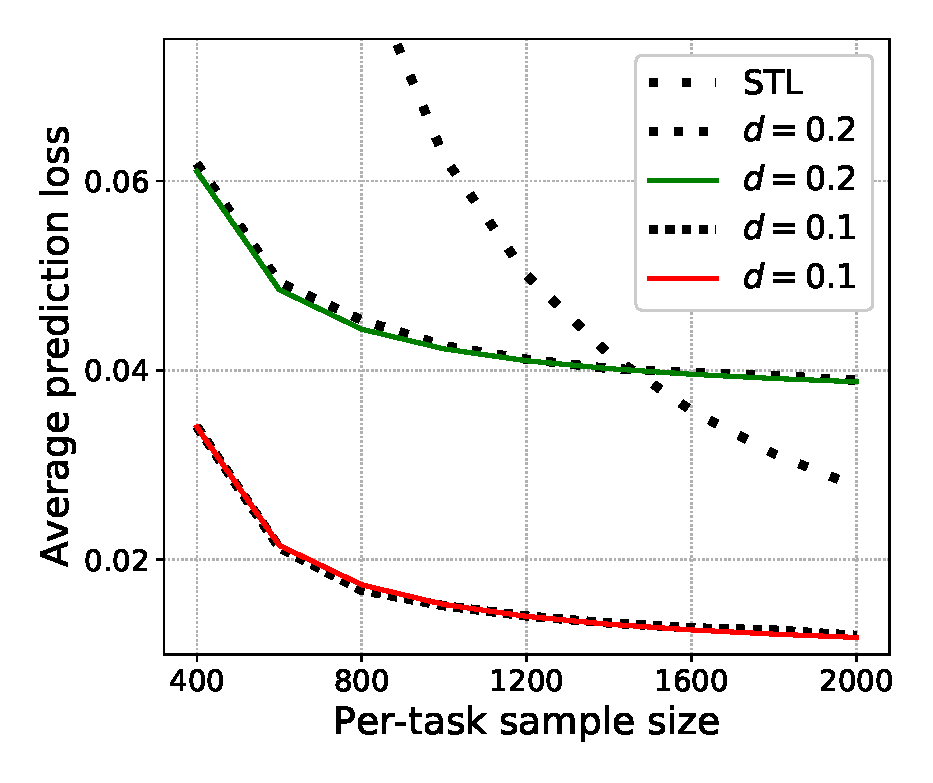
\includegraphics[width=0.98\textwidth]{figures/same_covariates.eps}
		\caption{Example \ref{ex_same_cov}}
		\label{fig_same_cov}
	\end{subfigure}\hfill
	\begin{subfigure}[b]{0.33\textwidth}
		\centering
		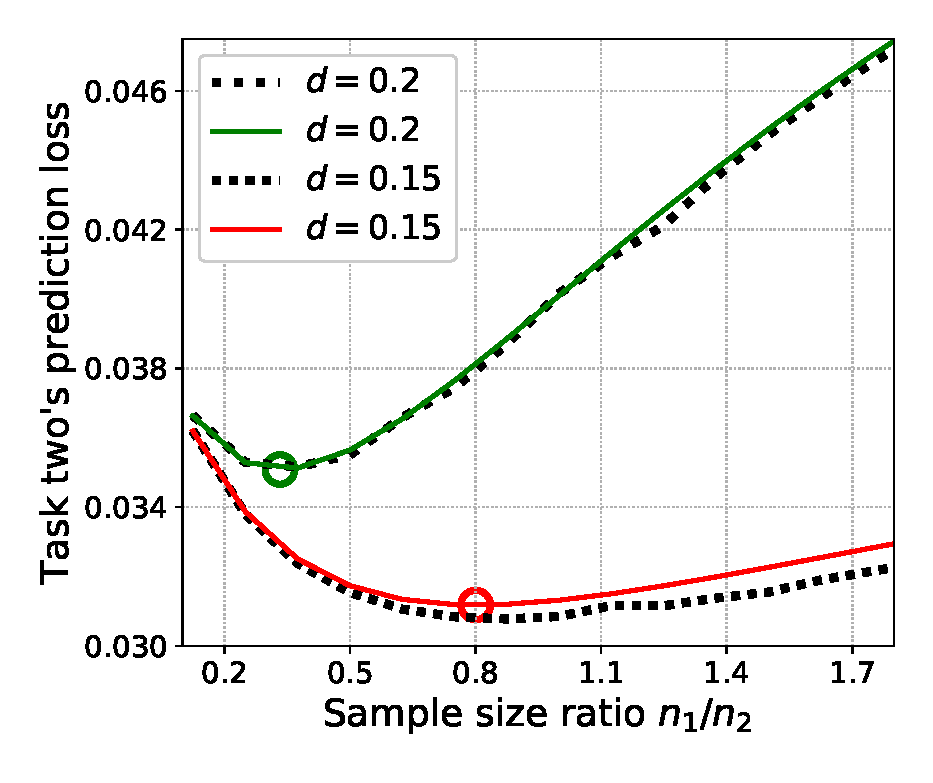
\includegraphics[width=0.98\textwidth]{figures/sample_ratio_several_d.eps}
		\caption{Example \ref{ex_sample_ratio}}
		\label{fig_size}
	\end{subfigure}\hfill
	\begin{subfigure}[b]{0.33\textwidth}
		\centering
		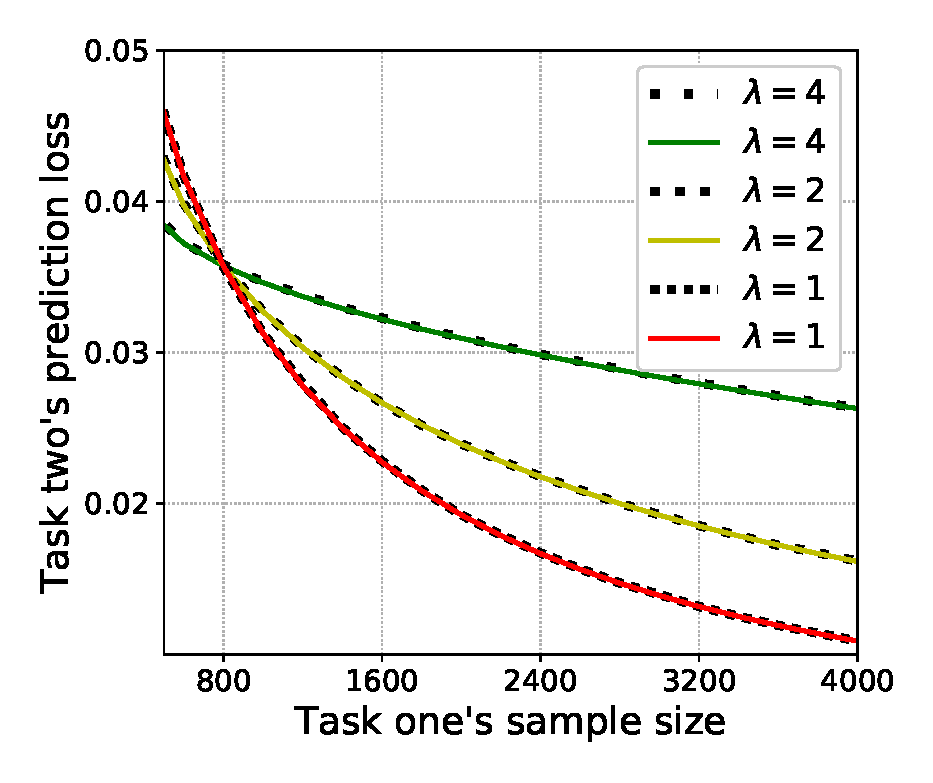
\includegraphics[width=0.98\textwidth]{figures/covariate_shift.eps}
		\caption{Example \ref{ex_covshift}}
		\label{fig_covariate}
	\end{subfigure}
	\caption{%Three takeaways of our theory in Section \ref{sec_insight}.
	Our estimated losses (solid line) match the empirical losses (dotted line) accurately under various settings in dimension $p = 200$.
	\textbf{Left.} Validating Example \ref{ex_same_cov} for ten tasks: the noise variance $\sigma^2$ is $1/4$.
	\textbf{Middle.} Validating Example \ref{ex_sample_ratio} for two tasks: we discover an interesting phenomena by fixing task two's sample size and increasing task one's sample size.
	Moreover, our result accurately predicts the critical point (marked in circle) of the loss curve.
%	Depending on how large the distance $d^2$ is, task two's prediction loss decreases initially before increasing again, or decreases monotonically.
	\textbf{Right.} We show how different levels of covariate shift affect hard parameter sharing when there is no bias.
	Having covariate shift increases task two's prediction loss when task two's sample size is smaller than task one. Otherwise, having covariate shift (surprisingly) decreases task two's prediction loss.}
	\label{fig_model_shift_phasetrans}
\end{figure*}



\paragraph{Sample efficiency}
First, we validate the result of Example \ref{ex_same_cov}.
Figure \ref{fig_same_cov} shows the average prediction loss over ten tasks as we increase the number of samples per-task from $400$ to $2000$.
In all the parameter settings, our results estimate the empirical losses accurately.
We also observe a trend that the average prediction loss increases as we increase distance $d$ from $0.1$ to $0.2$.
Our work explains the differences between these two settings since $d^2 = 0.1^2$ is always smaller than $\frac{\sigma^2 p}{n - p}$, but $d^2 = 0.2^2$ is not.
%Second, when $d = 0.1$, we have that $d^2 \le \frac{\sigma^2 p}{n - p}$ for all values of $n$, hence the average prediction loss of hard parameter sharing is always lower than STL.
Indeed, we observe a crossover point between hard parameter sharing and STL.
Finally, for $d = 0.2$, looking horizontally, we find that HPS requires fewer samples per-task than STL to achieve the same loss level. %\FY{I do not quite understand this sentence about "3x fewer", because how much data needed depends on $d$ and the prediction loss level we are looking at. For example, at the cross point, this ratio is 1. }

\paragraph{Sample size ratio}
Second, we validate the result of Example \ref{ex_sample_ratio}.
Figure \ref{fig_size} shows task two's prediction loss  as we increase the sample ratio $n_1 / n_2$ from $1/10$ to $7/10$.
%Again, our estimates are accurate compared to the empirical losses.
We consider a regime where task two consists of $80,000$ samples, and task one's sample size varies from $8,000$ to $56,000$.
The task-specific variance (which scales with model distance) is $d = 0.2$, the noise variance is $\sigma^2 = 4^2$, and the shared signal variance is $1$. We observe that as we increase the sample ratio, task two's prediction loss decreases initially but later will increase when the sample ratio is above a certain level.
On the other hand, when $d = 0.15$, task two's prediction loss decreases faster.
Intuitively, this is because bias increases less for smaller $d^2$.
%Our result from Corollary \ref{cor_MTL_loss} explains this trend.

\paragraph{Covariate shift}
Finally, we validate the result of Example \ref{ex_covshift}.
Figure \ref{fig_covariate} shows task two's prediction loss as we increase task one's sample size.
Recall that $\lambda$ measures the severity of covariate shifts---a larger $\lambda$ means a larger covariate shift.
We indeed observe the dichotomy in Example \ref{ex_covshift} at $n_1 = 800$.
The sample size $n_2$ is $800$ and the noise variance $\sigma^2$ is $1/4$.
%Covariate shift: We set $\kappa = 1$ and $d = 0$.
%We set $\rho_2 = 4$ and vary $\rho_1$ from $5$ to $25$ for sample sizes.
%We use the scale parameter $\lambda = 1$ for the curve without covariate shift and $\lambda = 2$ for the curve with covariate shift (cf. Section \ref{sec_covshift}).


%Recall that Section \ref{sec_data_size} shows that increasing the data size of the source task does not always improve the performance of MTL for the target task.
%In Figure \ref{fig_ab_data}, we show that for source task MR and target task SST, there is a transition from positive to negative transfer as we increase the data size of the source task.
%Our result provides a fine-grained insight on the covariance alignment algorithm proposed in \cite{WZR20}.
%Recall that the covariance alignment procedure in \cite{WZR20} adds an additional module between the word embedding representation and the shared module.
%When the source task data size is particularly large compared to the target task, we show that applying the covariance alignment algorithm results in more significant gains.
%In Figure \ref{fig_ab_cov}, we observe that the benefit from aligning task covariances becomes more significant for LSTM and MLP as we increase the number of datapoints of the source task.

%\begin{table}
%	\begin{center}
%		\begin{tabular}{c c c c c}
%			\toprule
%			\multirow{2}{*}{{\bf Models}} & \multicolumn{2}{c}{\begin{minipage}{1.1in}\begin{center}
%				                                                                          MR, SST, SUBJ, CR, MPQA, TREC\end{center}\end{minipage}} & \multicolumn{2}{c}{\begin{minipage}{1.1in}\begin{center}MR, SST, SUBJ, CR, MPQA\end{center}\end{minipage}} \\
%			\cmidrule(lr){2-3} \cmidrule(lr){4-5}
%			& {\bf Stanford} & {\bf Alignment} & {\bf Stanford} & {\bf Alignment} \\
%			\midrule
%			{\bf MLP}  & > 100\% & 39\% & 25\% & 25\% \\
%			{\bf LSTM} & 36\% & 36\% & 28\% & 25\% \\
			% {\bf CNN}  & 76\% & - & 32\% & -\\
%			\bottomrule
%		\end{tabular}
%	\end{center}
%	\caption{Taskonomy experiment.}
%	\label{tab:taskonomy}
%\end{table}
%\begin{figure}[!t]
%	\centering
%	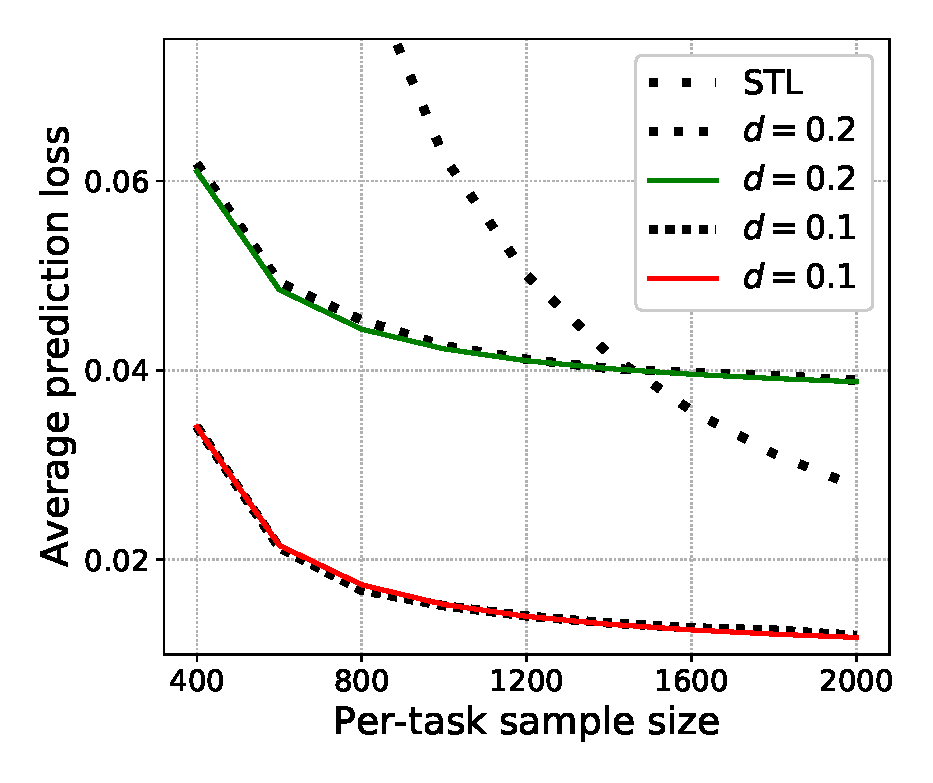
\includegraphics[width=0.35\textwidth]{figures/same_covariates.eps}
%	\caption{Validating Example \ref{ex_same_cov} in Section \ref{sec_same} for $10$ tasks: our estimated loss (solid line) matches the empirical loss (dotted line) accurately for various task-specific variance $d^2$ and sample size $n$ settings. The feature dimension $p$ is $200$, and noise variance $\sigma^2$ is $1/4$.}
%	\label{fig_same_cov}
%\end{figure}




